\documentclass[11pt,letterpaper]{article}
\usepackage[lmargin=1in,rmargin=1in,tmargin=1in,bmargin=1in]{geometry}
\usepackage{../style/homework}
\usepackage{../style/commands}
\setbool{quotetype}{true} % True: Side; False: Under
\setbool{hideans}{false} % Student: True; Instructor: False

% -------------------
% Content
% -------------------
\begin{document}

\homework{8: Due 10/29}{The world is a stage, but the play is badly cast.}{Oscar Wilde}

% Problem 1
\problem{10} Plot the quadratic function $y= 2x^2 - 4x + 3$ as accurately as possible. Your sketch should include the vertex and axis of symmetry. 
	\[
	\fbox{
	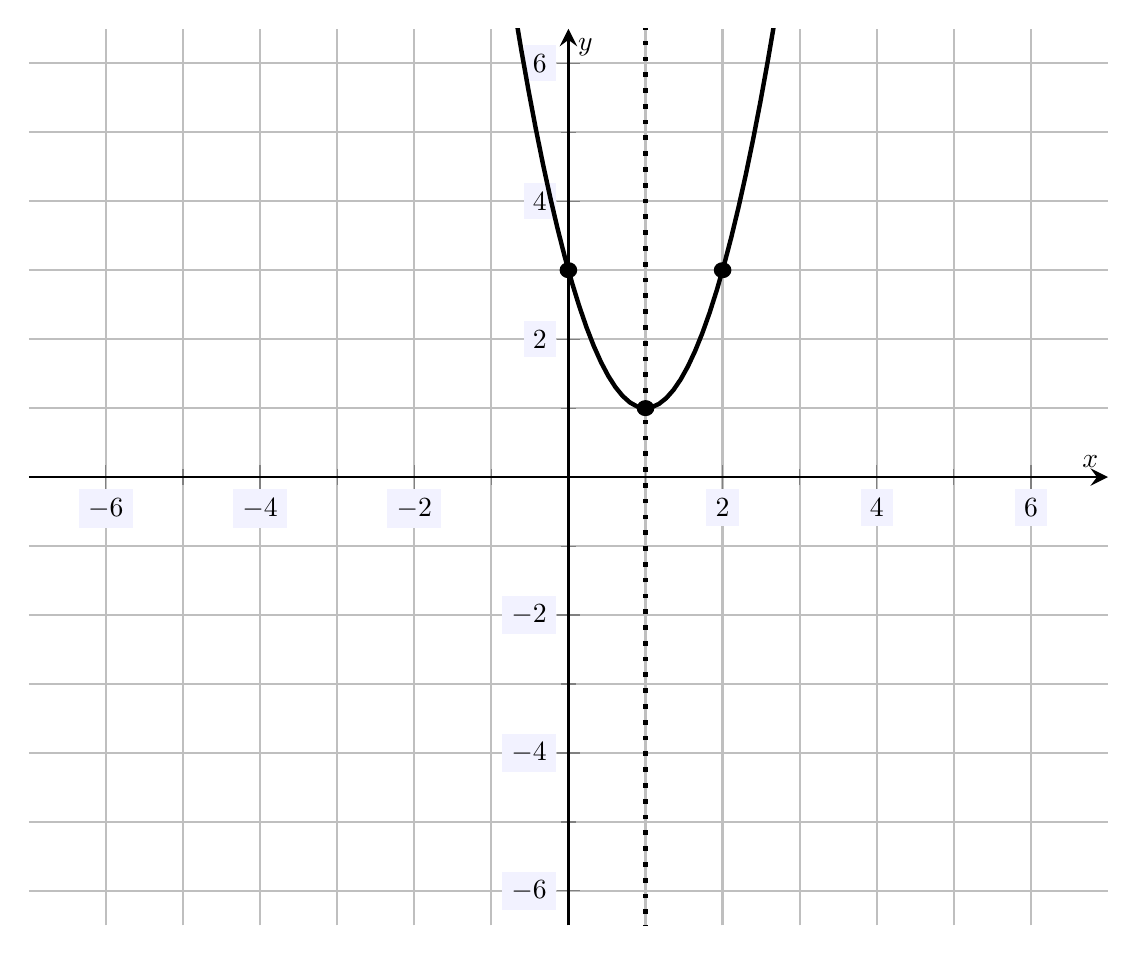
\begin{tikzpicture}[scale=2,every node/.style={scale=0.5}]
	\begin{axis}[
	grid=both,
	axis lines=middle,
	ticklabel style={fill=blue!5!white},
	xmin= -7, xmax=7,
	ymin= -6.5, ymax=6.5,
	xtick={-6,-4,-2,0,2,4,6},
	ytick={-6,-4,-2,0,2,4,6},
	minor tick = {-5,-3,...,5},
	xlabel=\(x\),ylabel=\(y\),
	]
	\addplot[thick, domain= -7:7,samples=150] {2*x^2 - 4*x + 3};
	\draw[dotted,line width= 0.03cm] (1,-10) -- (1,10);
	\draw[fill=black] (0,3) circle (0.1);
	\draw[fill=black] (1,1) circle (0.1);
	\draw[fill=black] (2,3) circle (0.1);
	\end{axis}
	\end{tikzpicture}
	}
	\] \pspace

Because $a= 2 > 0$, the parabola opens upwards, i.e. is convex. The vertex occurs at $x= -\frac{b}{2a}= -\frac{-4}{2(2)}= 1$. We know 
	\[
	y(1)= 2(1^2) - 4(1) + 3= 2 - 4 + 3= 1
	\]
Therefore, the vertex is $(1, 1)$. We need to include this point. The axis of symmetry is $x= 1$. We find serval other points:
	\begin{table}[!ht]
	\centering
	\begin{tabular}{r||rrrrrrrrr}
	$x$ & $-4$ & $-3$ & $-2$ & $-1$ & $0$ & $1$ & $2$ & $3$ & $4$ \\ \hline
	$f(x)$ & $51$ & $33$ & $19$ & $9$ & $3$ & $1$ & $3$ & $9$ & $19$
	\end{tabular}
	\end{table}





\newpage





% Problem 2
\problem{10} Plot the quadratic function $y= -x^2 - 6x - 5$ as accurately as possible. Your sketch should include the vertex and axis of symmetry. 
	\[
	\fbox{
	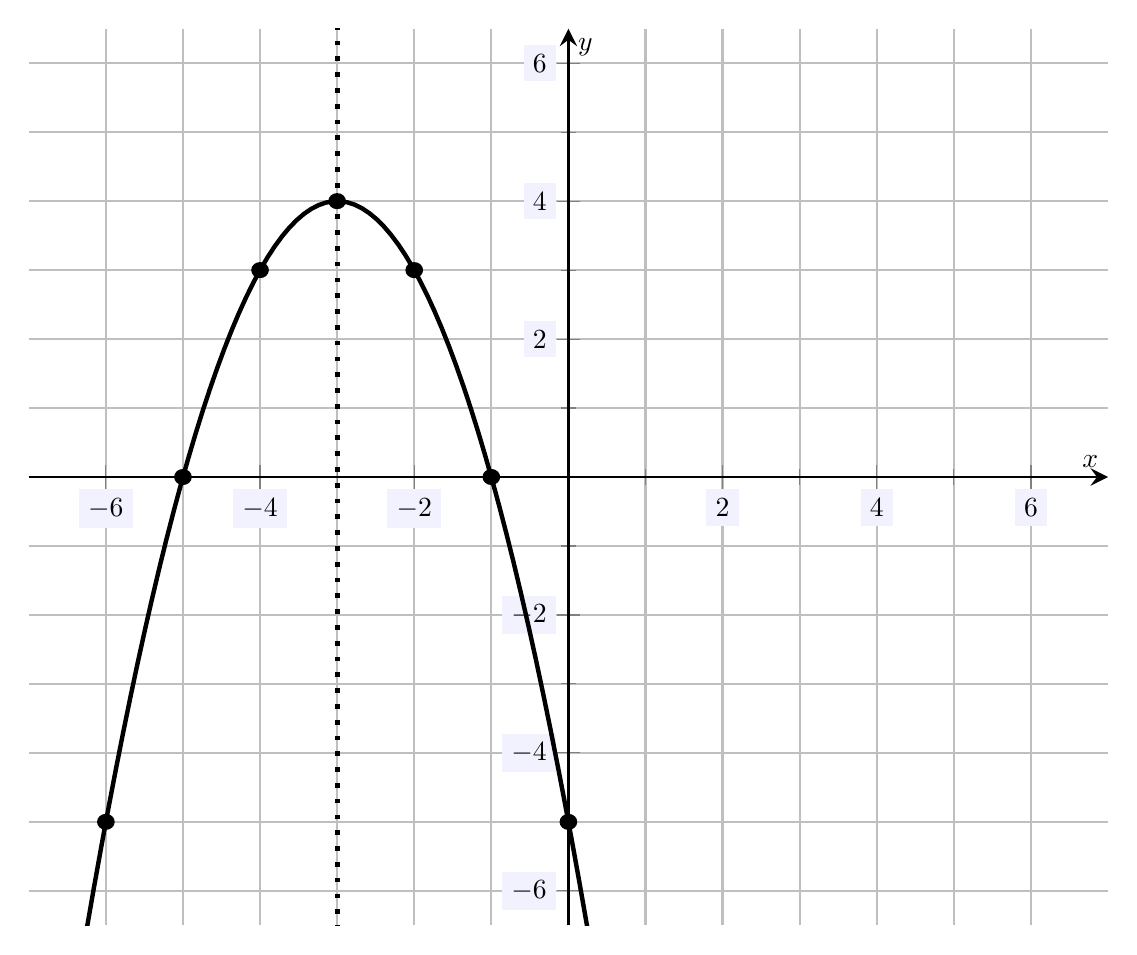
\begin{tikzpicture}[scale=2,every node/.style={scale=0.5}]
	\begin{axis}[
	grid=both,
	axis lines=middle,
	ticklabel style={fill=blue!5!white},
	xmin= -7, xmax=7,
	ymin= -6.5, ymax=6.5,
	xtick={-6,-4,-2,0,2,4,6},
	ytick={-6,-4,-2,0,2,4,6},
	minor tick = {-5,-3,...,5},
	xlabel=\(x\),ylabel=\(y\),
	]
	\addplot[thick, domain= -7:7,samples=150] {-1*x^2 - 6*x - 5};
	\draw[dotted,line width= 0.03cm] (-3,-10) -- (-3,10);
	\draw[fill=black] (-7,-12) circle (0.1);
	\draw[fill=black] (-6,-5) circle (0.1);
	\draw[fill=black] (-5,0) circle (0.1);
	\draw[fill=black] (-4,3) circle (0.1);
	\draw[fill=black] (-3,4) circle (0.1);
	\draw[fill=black] (-2,3) circle (0.1);
	\draw[fill=black] (-1,0) circle (0.1);
	\draw[fill=black] (0,-5) circle (0.1);
	\draw[fill=black] (1,-12) circle (0.1);
	\end{axis}
	\end{tikzpicture}
	}
	\] \pspace

Because $a= -1 < 0$, the parabola opens downwards, i.e. is concave. The vertex occurs at $x= -\frac{b}{2a}= -\frac{-6}{2(-1)}= -3$. We know 
	\[
	y(-3)= -(-3)^2 - 6(-3) - 5= -9 + 18 - 5= 4
	\]
Therefore, the vertex is $(-3, 4)$. We need to include this point. The axis of symmetry is $x= 1$. We find serval other points:
	\begin{table}[!ht]
	\centering
	\begin{tabular}{r||rrrrrrrrr}
	$x$ & $-7$ & $-6$ & $-5$ & $-4$ & $-3$ & $-2$ & $-1$ & $0$ & $1$ \\ \hline
	$f(x)$ & $-12$ & $-5$ & $0$ & $3$ & $4$ & $3$ & $0$ & $-5$ & $-12$
	\end{tabular}
	\end{table}





\newpage





% Problem 3
\problem{10} Give a rough sketch of the quadratic function $y= 2(x - 1)^2 + 3$. Your sketch should include the vertex and axis of symmetry. 
	\[
	\fbox{
	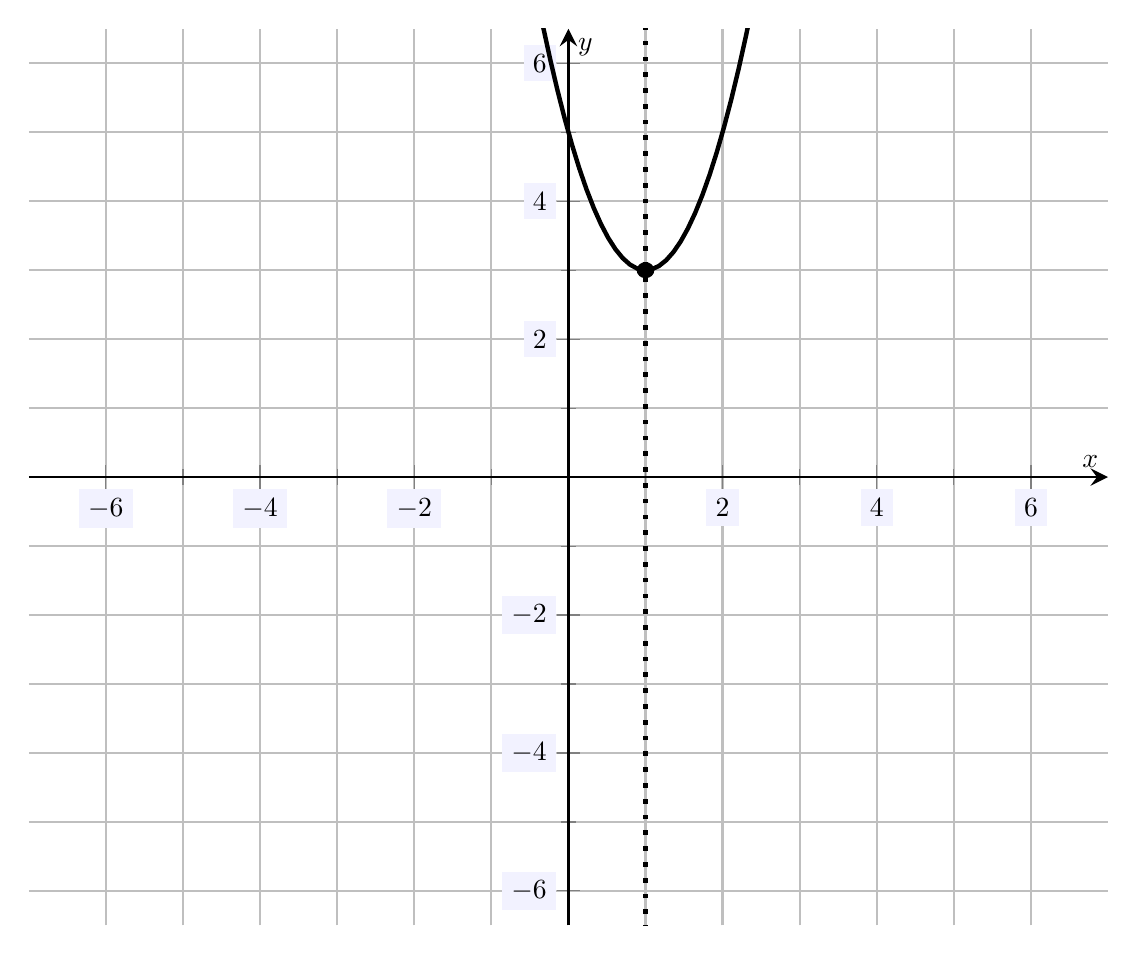
\begin{tikzpicture}[scale=2,every node/.style={scale=0.5}]
	\begin{axis}[
	grid=both,
	axis lines=middle,
	ticklabel style={fill=blue!5!white},
	xmin= -7, xmax=7,
	ymin= -6.5, ymax=6.5,
	xtick={-6,-4,-2,0,2,4,6},
	ytick={-6,-4,-2,0,2,4,6},
	minor tick = {-5,-3,...,5},
	xlabel=\(x\),ylabel=\(y\),
	]
	\addplot[thick, domain= -7:7,samples=150] {2*(x - 1)^2 + 3};
	\draw[dotted,line width= 0.03cm] (1,-10) -- (1,10);
	\draw[fill=black] (1,3) circle (0.1);
	\end{axis}
	\end{tikzpicture}
	}
	\] \pspace

Because $a= 2 > 0$, the parabola opens upwards, i.e. is convex. Because the parabola is in vertex form, we know the vertex is $(1, 3)$. Therefore, the axis of symmetry is $x= 1$. 





\newpage





% Problem 4
\problem{10} Give a rough sketch of the quadratic function $y= 4 - (x + 1)^2$. Your sketch should include the vertex and axis of symmetry.  
	\[
	\fbox{
	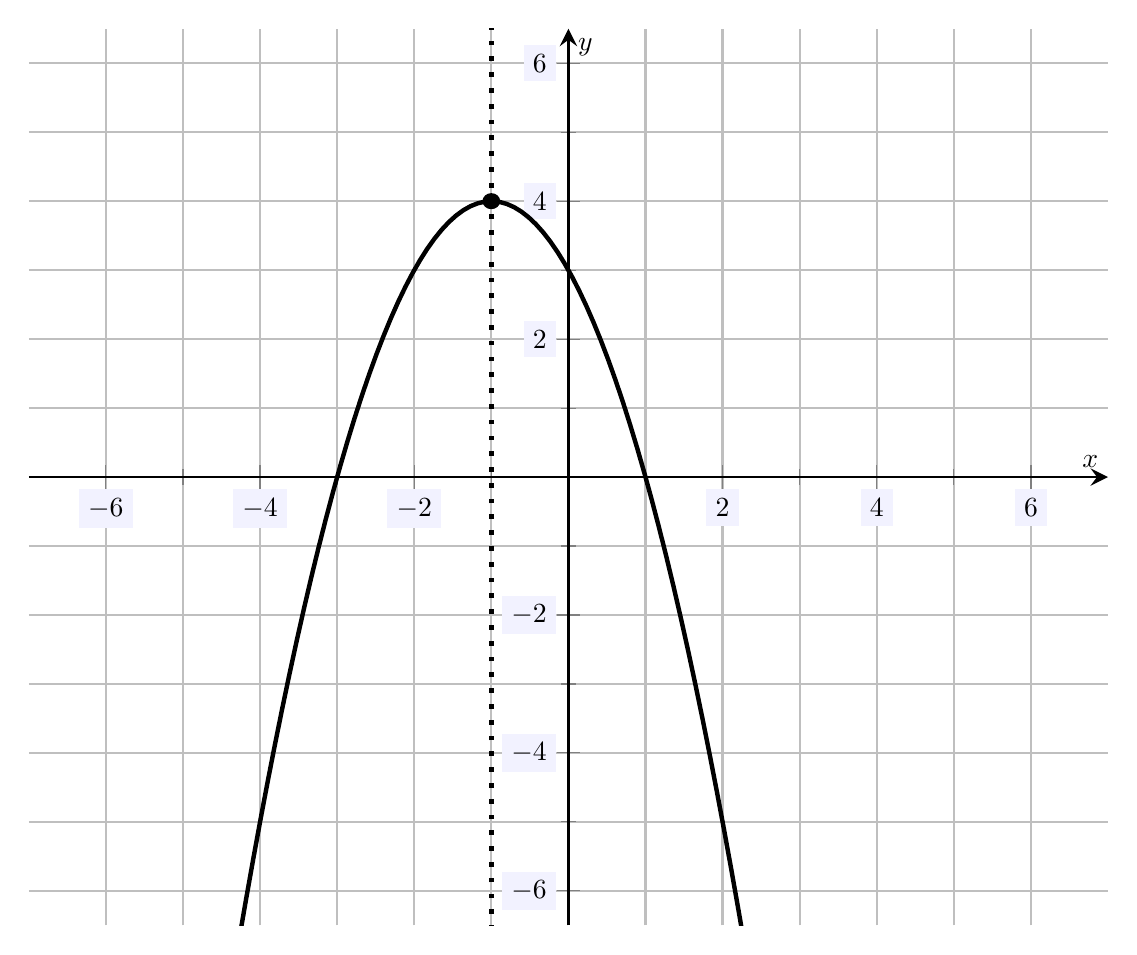
\begin{tikzpicture}[scale=2,every node/.style={scale=0.5}]
	\begin{axis}[
	grid=both,
	axis lines=middle,
	ticklabel style={fill=blue!5!white},
	xmin= -7, xmax=7,
	ymin= -6.5, ymax=6.5,
	xtick={-6,-4,-2,0,2,4,6},
	ytick={-6,-4,-2,0,2,4,6},
	minor tick = {-5,-3,...,5},
	xlabel=\(x\),ylabel=\(y\),
	]
	\addplot[thick, domain= -7:7,samples=150] {4 - (x + 1)^2};
	\draw[dotted,line width= 0.03cm] (-1,-10) -- (-1,10);
	\draw[fill=black] (-1,4) circle (0.1);
	\end{axis}
	\end{tikzpicture}
	}
	\] \pspace

Because $a= -1 < 0$, the parabola opens downwards, i.e. is concave. Because the parabola is in vertex form, we know the vertex is $(-1, 4)$. Therefore, the axis of symmetry is $x= -1$. 

%\printpoints
\end{document}